\documentclass[10pt]{beamer}
\mode<presentation> {
\usetheme{Darmstadt}
}
\usepackage{amssymb}
\usepackage{amsmath}
\usepackage{amsfonts}
\usepackage{bbm}
\usepackage{amsthm}
\usepackage{newtxmath}
\usepackage{graphics, graphicx}
\usepackage{float}
\usepackage{subcaption}
\usepackage{listings}
\usepackage{booktabs}
\usepackage{Sweave}
\usepackage{natbib}
\usepackage{bm}
\usepackage[font={small, it}]{caption}
\usepackage{wrapfig}
\usepackage{mathtools}
\usepackage{dsfont}
% \usepackage[round]{natbib}
\usepackage{multirow}
\usepackage{verbatim}
\usepackage{listings}




\usepackage[linesnumbered,ruled,vlined]{algorithm2e}
\usepackage{algpseudocode}  
\usepackage{algorithmic}
\usepackage{hyperref}
\hypersetup{
    colorlinks=true,
    linkcolor=white,
    filecolor=blue,      
    urlcolor=blue,
    citecolor=blue,
}


\newcommand{\cE}{\mathcal{E}}
\newcommand{\cX}{\mathcal{X}}
\newcommand{\cR}{\mathcal{R}}
\newcommand{\cV}{\mathcal{V}}
\newcommand{\bw}{\mathbf{w}}
\newcommand{\bb}{\mathbf{b}}
\newcommand{\bG}{\mathbf{G}}
\newcommand{\bu}{\mathbf{u}}
\newcommand{\bv}{\mathbf{v}}
\newcommand{\bH}{\mathbf{H}}
\newcommand{\be}{\mathbf{e}}
\newcommand{\bx}{\bm{x}}
\newcommand{\bbt}{\bm{\beta}}
\newcommand{\ty}{\tilde{y}}
\newcommand{\cA}{\mathcal{A}}
\newcommand{\bX}{\mathbf{X}}
\newcommand{\bDelta}{\bm{\Delta}}
\newcommand{\bB}{\mathbb{B}}


\setlength{\parindent}{0em}
\setlength{\parskip}{0.5em}
\renewcommand{\baselinestretch}{1.1}



%\usepackage[most]{tcolorbox}
%\tcbuselibrary{theorems}
%\newtcbtheorem{Definitions}{Definition}%
%{colframe=blue!70!black!,fonttitle=\bfseries}{}


 
%---------------------------------------------------------------------------------------
%	TITLE PAGE
%---------------------------------------------------------------------------------------

\title[\textcolor{white}{Crime Forecasting}]{Crime Forecasting using Satellite Imagery}
\author{He Zhou}
\institute[UMN] 
{University of Minnesota, 3rd Stats PhD}
\date{\today} 


\begin{document}

\begin{frame}[plain,noframenumbering]

\end{frame}

\begin{frame}[plain]
\titlepage 
\end{frame}




%----------------------------------------------------------------------------------------
%	PRESENTATION SLIDES
%----------------------------------------------------------------------------------------

%------------------------------------------------
\section{Introduction}

\begin{frame}{Crime Forecasting}
\begin{itemize}
    \item \textbf{Goal:} Predict future high-risk crime areas (hot spots) through past spatial and temporal information
    \item \textbf{Tasks:}
    \begin{itemize}
        \item Classification (hot spot forecasting): crime / no crime
        \item Prediction: number of crimes
    \end{itemize}
\end{itemize}
\end{frame}


\begin{frame}{Motivation: Examine Deep Learning Architectures}
\emph{``Examining Deep Learning Architectures for Crime Classification
and Prediction'' \citep{stalidis2021examining}}
\begin{columns}[onlytextwidth]
    \column{.47\textwidth}
        \begin{figure}
            \centering
            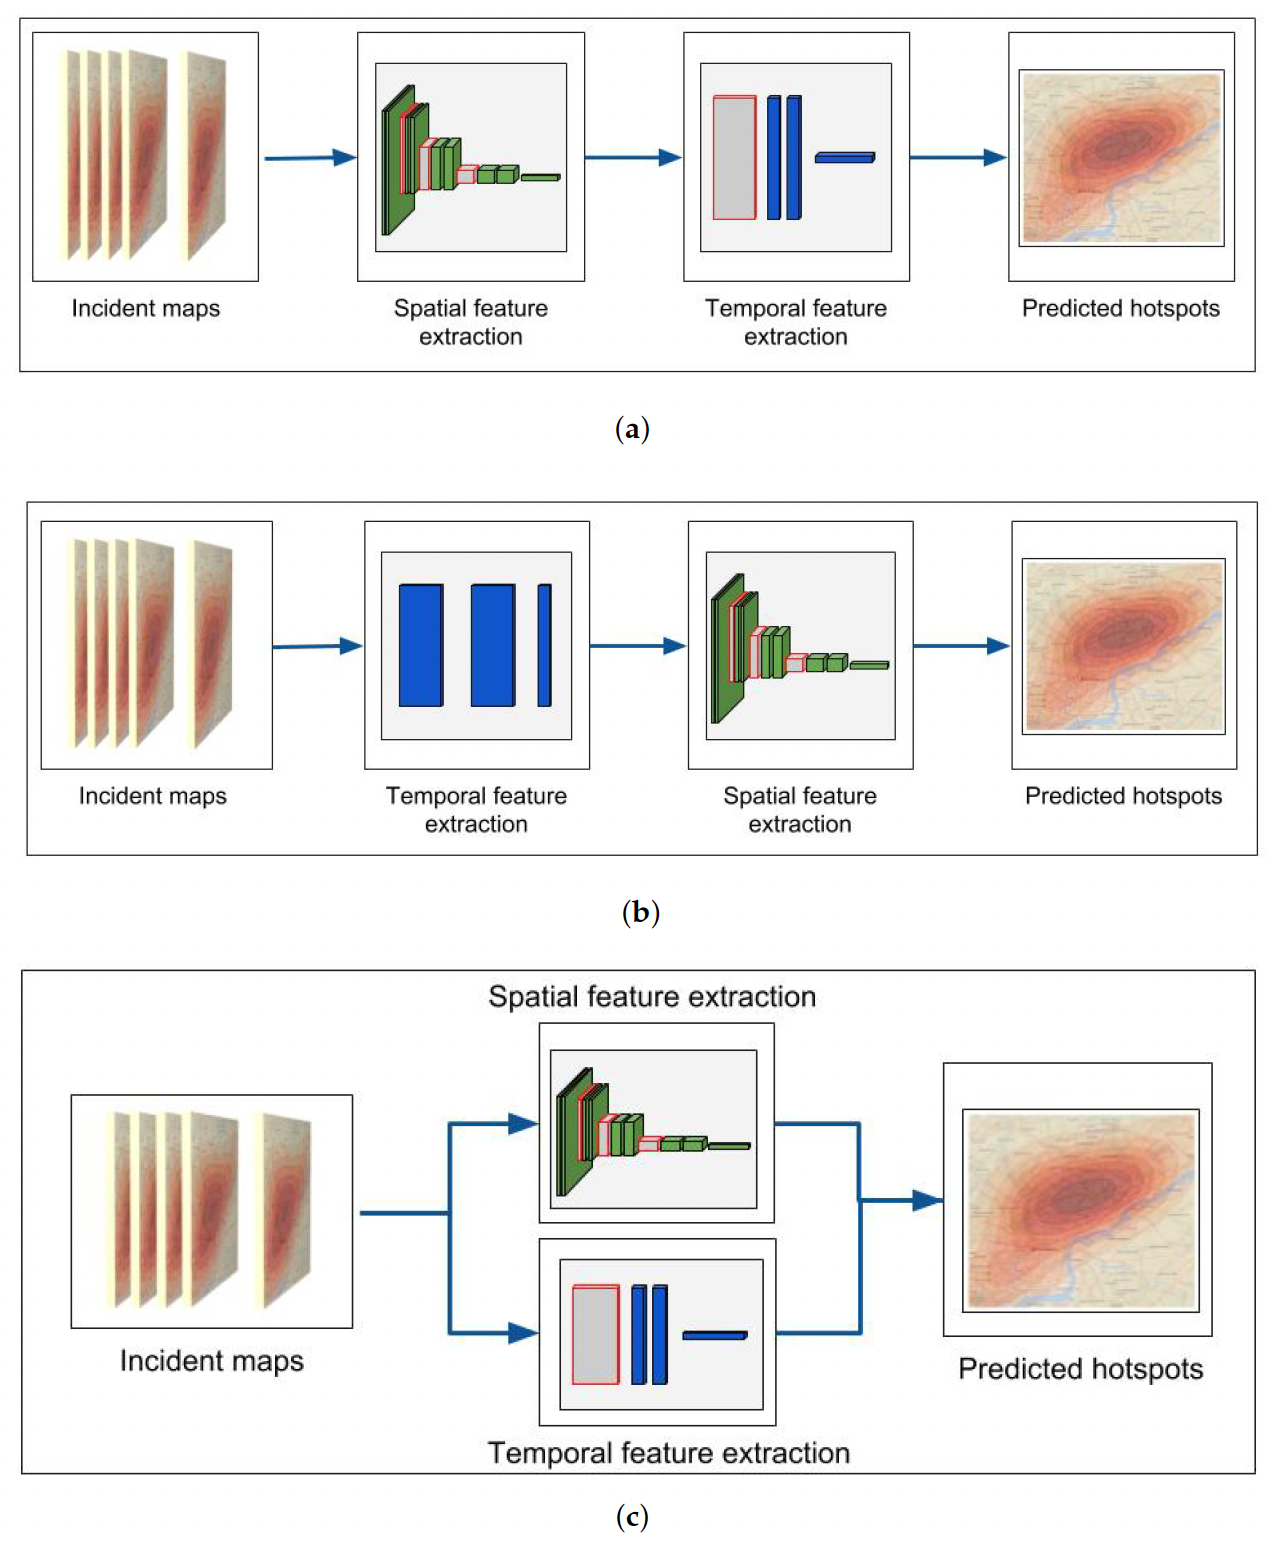
\includegraphics[width=1\textwidth]{ExamDL.png}
        \end{figure}
    \column{.47\textwidth}
        \begin{itemize}
            \item Use only \emph{location}, \emph{time}, \emph{crime type} from incident reports
            \item Crime classification and prediction simultaneously
        \end{itemize}
\end{columns}

\end{frame}

\begin{frame}{Motivation: Satellite Imagery}
\emph{``Crime Mapping from Satellite Imagery via Deep Learning'' \citep{najjar2018crime}}
\begin{figure}
\centering
\begin{subfigure}{.4\textwidth}
  \centering
  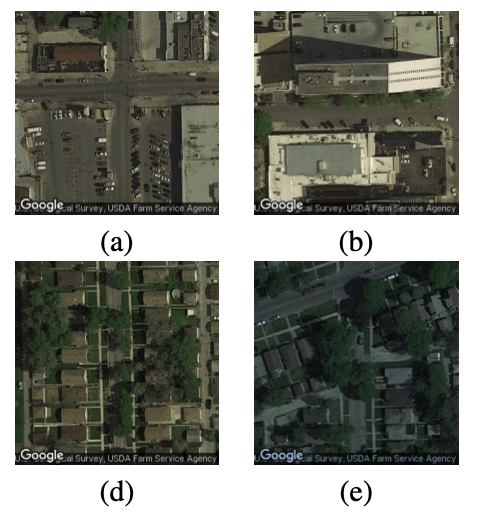
\includegraphics[width=0.75\linewidth]{Satellite_Images.png}
  \caption{Satellite images}
  \label{fig:sub1}
\end{subfigure}%
\begin{subfigure}{.6\textwidth}
  \centering
  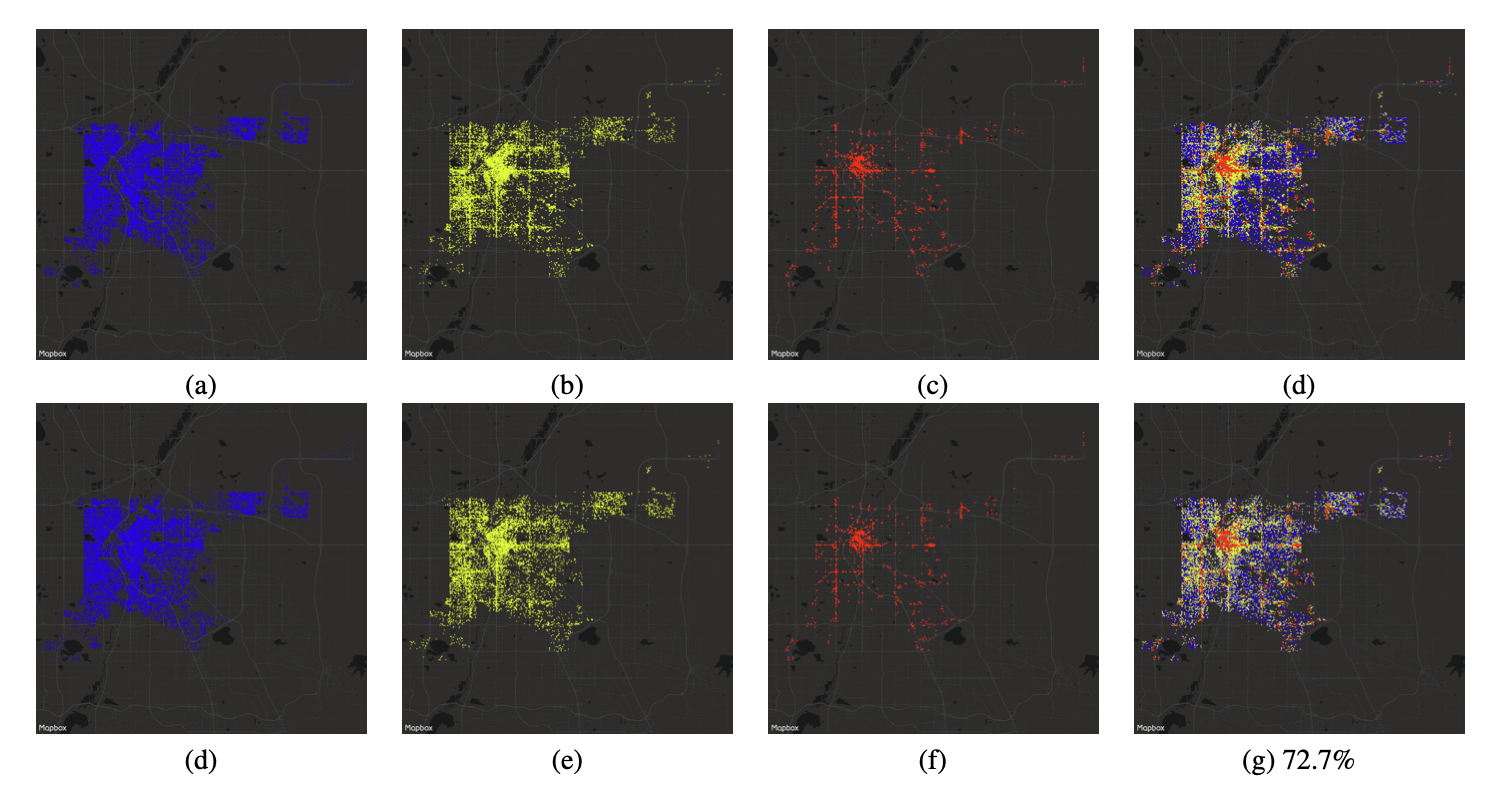
\includegraphics[width=1\linewidth]{Crime_Maps.png}
  \caption{Crime maps (Accuracy: $79\%$)}
  \label{fig:sub2}
\end{subfigure}
\caption{Visual features contained in satellite imagery can be used as a proxy indicator
of crime rates}
\label{fig:test}
\end{figure}
\end{frame}

\begin{frame}{Question}
\centering
{\large
\textbf{Question:} Forecast crime hotspots with satellite imagery?
}
\end{frame}

%------------------------------------------------


\section{Problem Formulation}
\begin{frame}{Problem Formulation}
\begin{itemize}
    \item \textbf{Incident Report Dataset:}
    \begin{itemize}
        \item Location: longitude \& latitude
        \item Time: year-month-day \& time
        \item Crime type: $C$ types
    \end{itemize}
    \item \textbf{Grid \citep{lin2018grid}:}
    \begin{itemize}
        \item cell edge size $\ell$
        \item $H \times W$ cells grid
    \end{itemize}
    \item \textbf{Aggregation:}
    \begin{itemize}
        \item Given timespan $t$, crime type $c$, cell $(i,j)$, 
        \item Count sum of occurences $y$.
        \item Multiple Incident Maps for period $T$: $(T, C, H, W)$
    \end{itemize}
    \item \textbf{Satellite Images:}
    \begin{itemize}
        \item For each cell $(i,j)$, get static map\footnote{Google Static Maps API: \url{https://developers.google.com/maps/documentation/static-maps}} centered around centroid
        \item pixels: $256\times 256$; zoom level: $17$
    \end{itemize}

    
\end{itemize}

\end{frame}



\section{Proposed Method}

\begin{frame}{Spatio-temporal Model: Dynamic Feature Extraction}
\emph{Examine Deep Learning Architectures for Crime Classification and Prediction \citep{stalidis2021examining}}

\begin{figure}
  \centering
    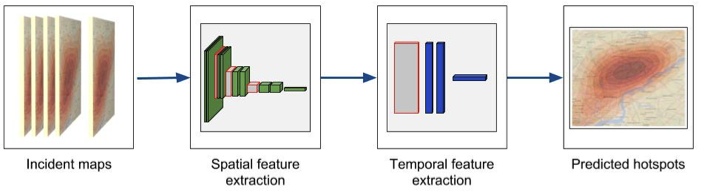
\includegraphics[width=1\textwidth]{SFTT_Feature_Extraction.png}
    \caption{Feature Extraction: the spatial features first then the temporal (SFTT).}
\end{figure}

\end{frame}

\begin{frame}{VGGNet : Spatial Feature Extraction}
\begin{figure}
  \centering
    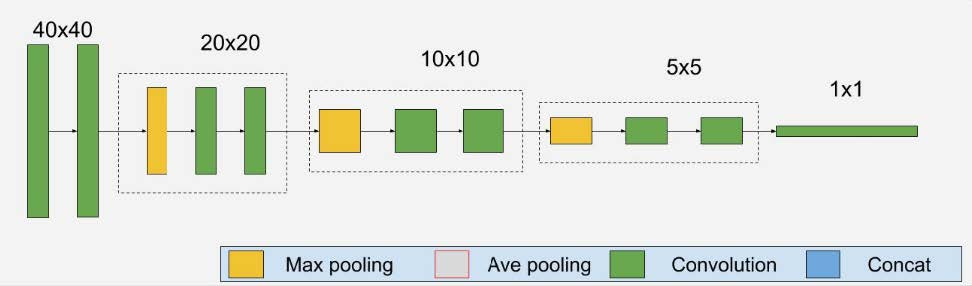
\includegraphics[width=0.8\textwidth]{VGGNet.jpg}
    \caption{VGGNet \citep{simonyan2014very}}
\end{figure}
{\small
\textbf{CNN Architecture:}
\begin{align*}
    \text{incident map}&\rightarrow
    (3\times 3\text{ conv}, 32) \times 2
    \overset{\text{pool}}{\rightarrow}
    (3\times 3\text{ conv}, 64) \times 2
    \\
    &
    \overset{\text{pool}}{\rightarrow}
    (3\times 3\text{ conv}, 128) \times 2
    \overset{\text{pool}}{\rightarrow}
    (3\times 3\text{ conv}, 256) \times 2
    \\
    &
    \rightarrow
    (1\times 1\text{ conv}, 256) \times 2
    \overset{\text{flatten}}{\rightarrow}
    \text{spatial features}
\end{align*}
}
\centering
{\footnotesize
\textbf{Remark:} Batch normalization and dropout layers used to avoid overfitting.
}


\end{frame}

\begin{frame}{LSTM : Temporal Feature Extraction}
\begin{figure}
  \centering
    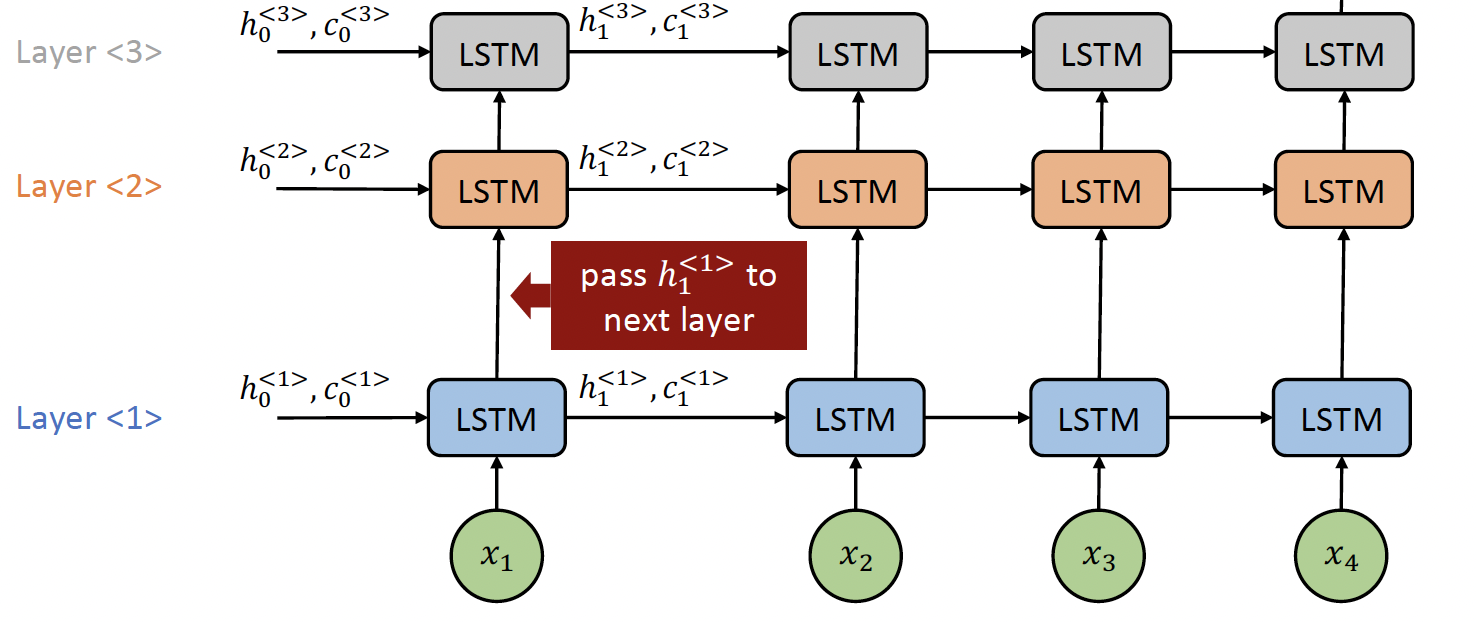
\includegraphics[width=0.8\textwidth]{Stacked_LSTMs.png}
    \caption{\footnote{Credit: \url{https://yaoyichi.github.io/spatial-ai.html}} Stacked LSTMs \citep{hochreiter1997long}}
\end{figure}
\begin{itemize}
    \item $x_t$: spatial features
    \item $h_t^{<1>}\in \mathbb{R}^{500}$, $h_t^{<2>}\in \mathbb{R}^{500}$, $h_t^{<3>}\in \mathbb{R}^{N}$
    \item $(h_1^{<3>}, \cdots, h_T^{<3>})$: dynamic spatio-temporal features
\end{itemize}
\end{frame}

\begin{frame}{AlexNet: Static Feature Extraction}
\begin{figure}
  \centering
    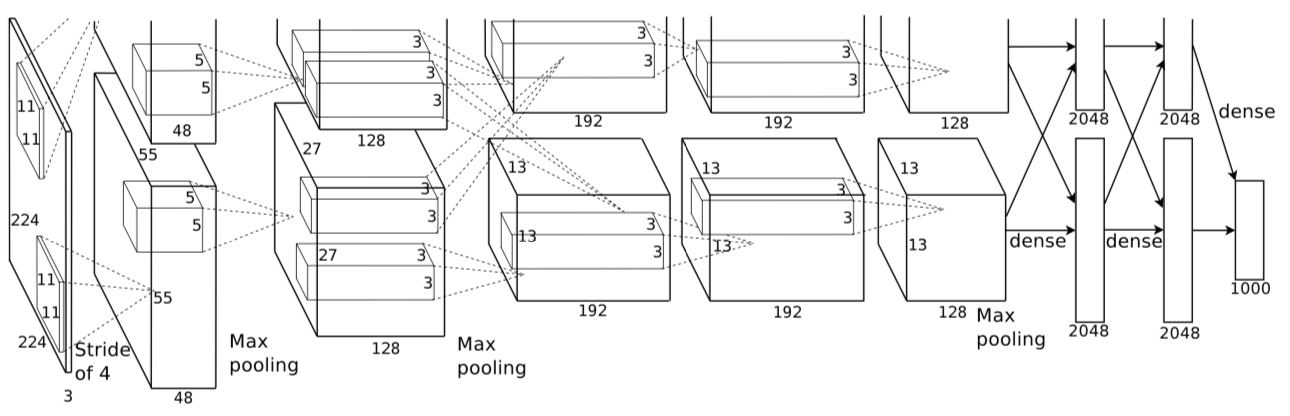
\includegraphics[width=0.8\textwidth]{AlexNet.png}
    \caption{AlexNet \citep{krizhevsky2012imagenet} as Static Feature Extractor}
\end{figure}
\begin{itemize}
    \item $s_{(i,j)}\in\mathbb{R}^{3\times 256\times256}$: satellite image centered at centroid of cell $(i,j)$
    \item $f_{(i,j)}\in\mathbb{R}^{1000}$: static features extracted by pre-trained AlexNet
    \item concatenate static features with the dynamic features
    \item feed into fully connected output layers
\end{itemize}
\end{frame}

\begin{frame}{Model Architecture}
\begin{figure}
  \centering
    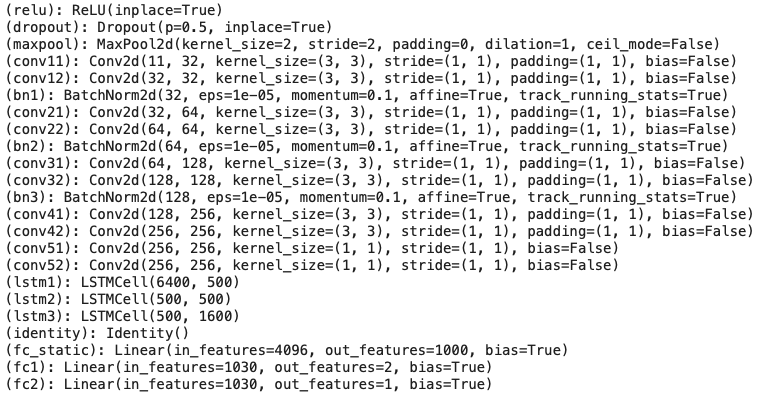
\includegraphics[width=0.8\textwidth]{Model_architecture.png}
    \caption{Model Architecture with $34,666,013$ parameters}
\end{figure}

\end{frame}



\begin{frame}{Custom Loss}
\begin{itemize}
    \item \textbf{Classification Loss:} Binary cross-entropy (BCE) loss
    \begin{equation*}
        BCE=-\frac{1}{N}\sum_{i=1}^{N}[\hat{o}_i\log o_i+(1-\hat{o}_i)\log(1-o_i)]
    \end{equation*}
    \item \textbf{Prediction Loss:} Mean squared error (MSE) loss
    \begin{equation*}
        MSE = \frac{1}{N}\sum_{i=1}^{N}(y_i-\hat{y}_i)^2
    \end{equation*}
    \item \textbf{Total Loss:} 
    \begin{equation*}
        Loss = BCE + \lambda \cdot MSE
    \end{equation*}
    where $\lambda$ is the regularization parameter for $MSE$.
\end{itemize}
\end{frame}


\section{Datasets}

\begin{frame}{San Francisco Incident Report}
\begin{figure}
  \centering
  \caption{Data table preview: San Francisco Police Department Incident Reports\footnote{\url{https://data.sfgov.org/Public-Safety/Police-Department-Incident-Reports-2018-to-Present/wg3w-h783}} (2018 to Present)}
    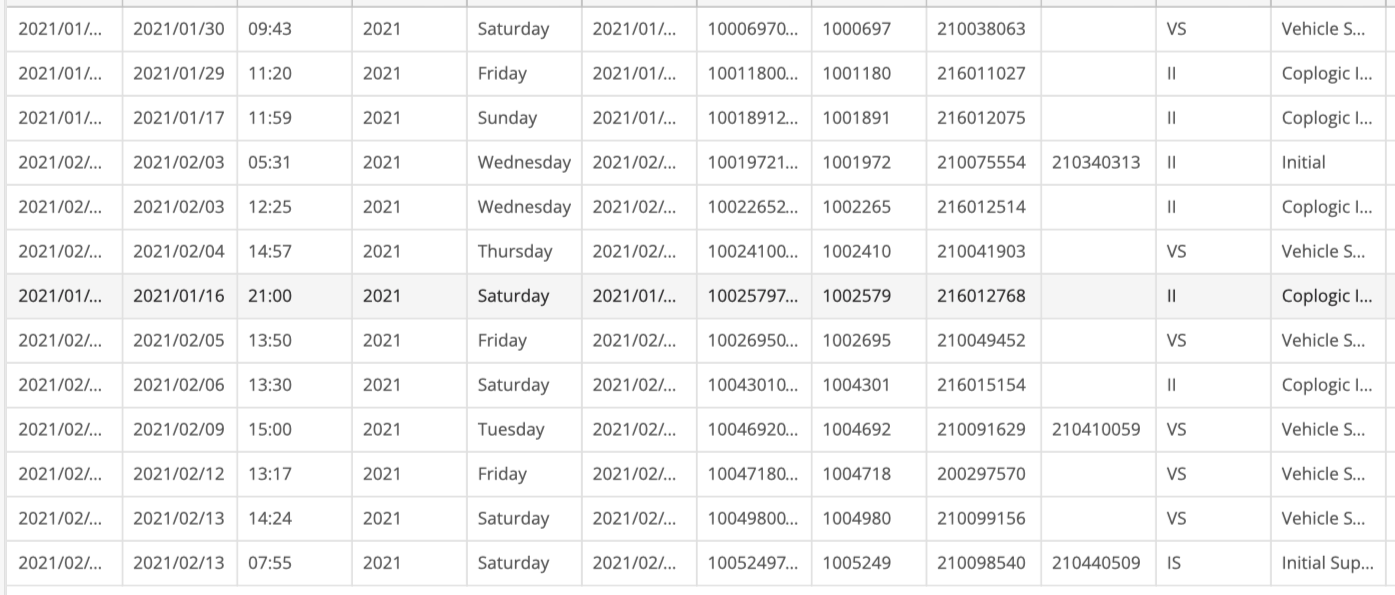
\includegraphics[width=0.7\textwidth]{SF_dataset.png}
\end{figure}
{\small
\begin{itemize}
    \item Start year: 2018 - End year: 2022
    \item 1572 days, 52 months
    
\end{itemize}
}
\end{frame}

\begin{frame}{San Francisco Incident Report}
Crime Types: \{Assault, Theft, Robbery, Burglary, Motor Vehicle, Arson, Homicide, Vice, Narcotics, Other\}
\begin{table}[h!]
\centering
\caption{Mapping of $47$ Crime Categories to the $10$ Crime Types \citep{stalidis2021examining}.}
{\footnotesize
 \begin{tabular}{ll} 
 \toprule
 \textbf{Crime Type} & \textbf{Crime Category} \\ [0.5ex] 
 \midrule
 \multirow{6}{}{Assault} & Assault  \\ 
 &Disorderly Conduct\\
 &Offences Against The Family And Children\\
 &Weapons Carrying Etc\\
 &Weapons Offence\\
 &Weapons Offense\\
 \hline
 \multirow{4}{}{Theft} & Larceny Theft \\
 &Malicious Mischief\\
 &Stolen Property\\
 &Vandalism\\
 \hline
 Robbery & Robbery \\
 \hline
 $\cdots$ & $\cdots$\\
 \bottomrule
 \end{tabular}
 }
 \end{table}
 
\end{frame}





\begin{frame}{San Francisco Incident Report}
\begin{table}[h!]
\centering
\caption{Column 2: Number of Incidents for each crime type;
\\Column 3: Mean number of hotspots per day for every crime type with $40\times 40$ cell grids.}
{\small
 \begin{tabular}{crr} 
 \toprule
 \textbf{Crime Type} & \textbf{Num. of Incidents} & \textbf{Mean Num. of hotspots}\\ [0.5ex] 
 \midrule
Assault & 59,773 &  27.78\\ 
 Theft & 202,506 & 93.77\\
 Robbery & 13,106 & 7.33\\
 Burglary & 32,816  & 17.99\\
 Motor Vehicle & 45,034  & 25.67\\
 Arson & 2,464 & 1.46\\
 Homicide & 64 & 0.04\\
 Vice & 1,791 & 0.79\\
 Narcotics & 13,564 & 4.48\\
 Other & 143,169 & 62.57\\
 \midrule
 Total & 514,287 & \# CELLS~~951\\ [1ex] 
 \bottomrule
 \end{tabular}
 }
 \end{table}
 
\end{frame}


\begin{frame}{San Francisco Satellite Images}
\begin{figure}
\centering
\begin{subfigure}{.35\textwidth}
  \centering
  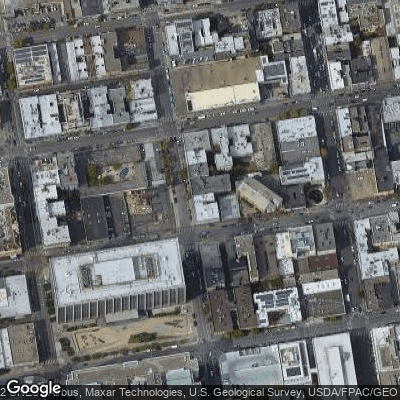
\includegraphics[width=0.7\linewidth]{985.png}
  \caption{Cell 985 with 9,194 incidents}
  \label{fig:sub1}
\end{subfigure}%
\begin{subfigure}{.35\textwidth}
  \centering
  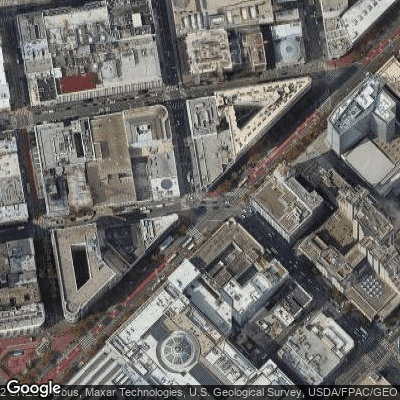
\includegraphics[width=0.7\linewidth]{1028.png}
  \caption{Cell 1028 with 7,779 incidents}
  \label{fig:sub2}
\end{subfigure}

\begin{subfigure}{.35\textwidth}
  \centering
  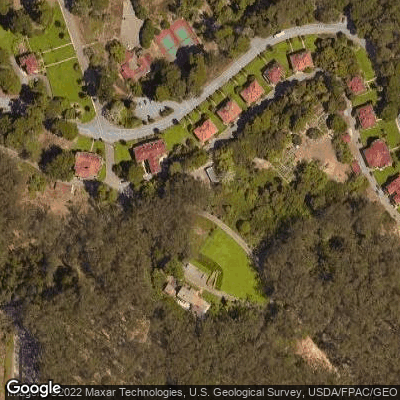
\includegraphics[width=0.7\linewidth]{1170.png}
  \caption{Cell 1170 with 1 incidents}
  \label{fig:sub1}
\end{subfigure}%
\begin{subfigure}{.35\textwidth}
  \centering
  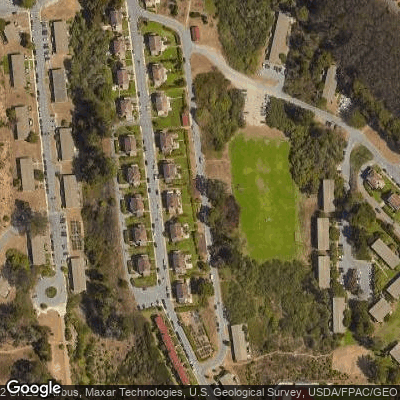
\includegraphics[width=0.7\linewidth]{1135.png}
  \caption{Cell 1135 with 1 incidents}
  \label{fig:sub2}
\end{subfigure}
\caption{Satellite images of four cells with high}
\label{fig:test}
\end{figure}
 
\end{frame}









\section{Experiment and Results}

\begin{frame}{Experimental Settings}
\begin{itemize}
    \item Grid: 
    \begin{itemize}
        \item cell edge size $\ell\approx 450$ m
        \item $40 \times 40$ cells grid
    \end{itemize}
    \item Aggregation:
    \begin{itemize}
        \item timespan $t$: 1 day
        \item period $T$: 30 days
        \item Incident maps: $(30, 10, 40, 40)$
    \end{itemize}
    \item Training:
    \begin{itemize}
        \item First $39$ periods for training and last $13$ for testing
        \item Loss regularization parameter $\lambda$: tune for different crime types
        \item Optimizer: $SGD$
        \item Training: $batch\_size=3$, $epoch=100$
    \end{itemize}
\end{itemize}


\end{frame}

% \begin{frame}{Training}
% \begin{figure}
%   \centering
%     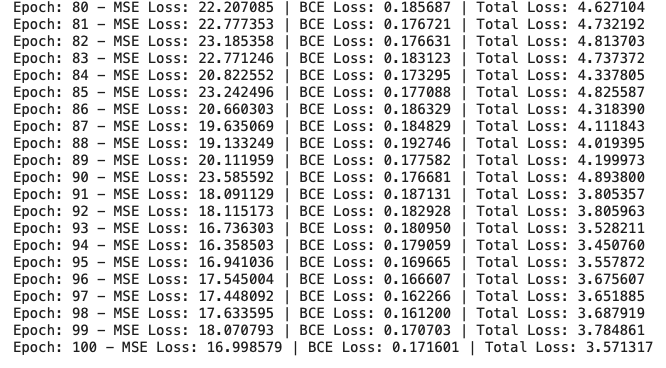
\includegraphics[width=0.8\textwidth]{loss_80_100.png}
%     \caption{Training outputs for the last 20 epochs.}
% \end{figure}
% 
% \end{frame}




\begin{frame}{Results}
\begin{figure}
\centering
\begin{subfigure}{.5\textwidth}
  \centering
  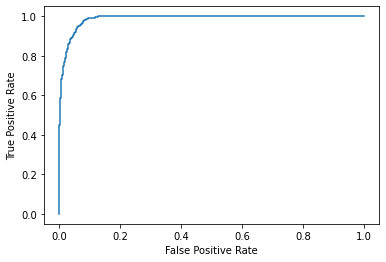
\includegraphics[width=0.7\linewidth]{ROC.png}
  \caption{All Crime ROC Curve \\
  (auroc = $0.989$)}
  \label{fig:sub1}
\end{subfigure}%
\begin{subfigure}{.5\textwidth}
  \centering
  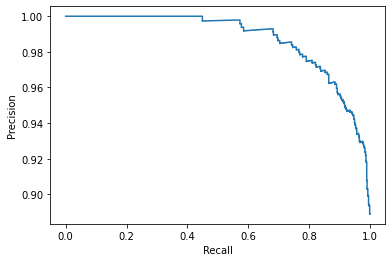
\includegraphics[width=0.7\linewidth]{PRC.png}
  \caption{All Crime Precision-Recall Curve \\
  (aps = $0.988$)}
  \label{fig:sub2}
\end{subfigure}

\begin{subfigure}{.5\textwidth}
  \centering
  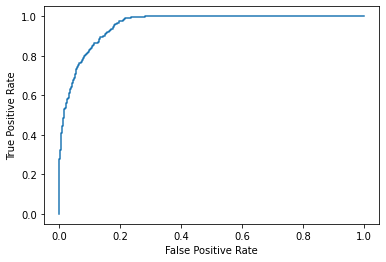
\includegraphics[width=0.7\linewidth]{ROC_theft.png}
  \caption{Theft ROC Curve \\
  (auroc = $0.957$)}
  \label{fig:sub1}
\end{subfigure}%
\begin{subfigure}{.5\textwidth}
  \centering
  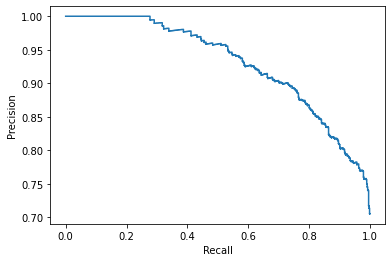
\includegraphics[width=0.7\linewidth]{PRC_theft.png}
  \caption{Theft Precision-Recall Curve \\
  (aps = $0.934$)}
  \label{fig:sub2}
\end{subfigure}
\label{fig:test}
\end{figure}
\end{frame}

\begin{frame}{Results}

\begin{figure}[!htb]
{\tiny
    \centering
    \begin{subfigure}{.32\textwidth}
        \centering
        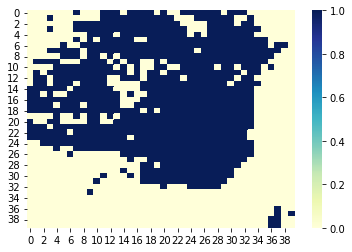
\includegraphics[width=1\linewidth, height=0.3\textheight]{true_hotspots.png}
        \caption{All crime true hotspots}
    \end{subfigure}%
    \begin{subfigure}{0.32\textwidth}
        \centering
        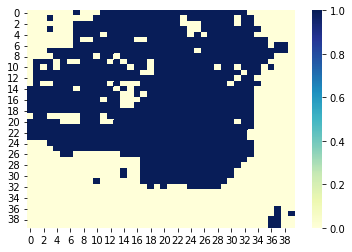
\includegraphics[width=1\linewidth, height=0.3\textheight]{pred_hotspots.png}
        \caption{pred. hotspots}
    \end{subfigure}%
    \begin{subfigure}{0.32\textwidth}
        \centering
        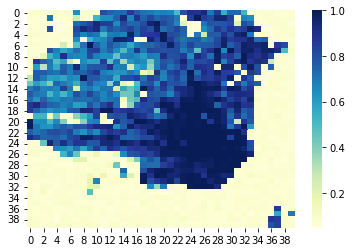
\includegraphics[width=1\linewidth, height=0.3\textheight]{pred_prob.png}
        \caption{pred. prob.}
    \end{subfigure}
    
    
    \begin{subfigure}{.32\textwidth}
        \centering
        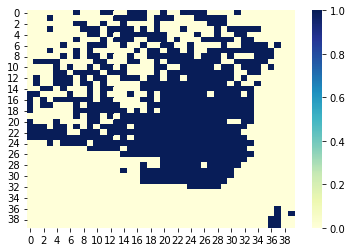
\includegraphics[width=1\linewidth, height=0.3\textheight]{true_theft_hotspots.png}
        \caption{Theft true hotspots}
    \end{subfigure}%
    \begin{subfigure}{0.32\textwidth}
        \centering
        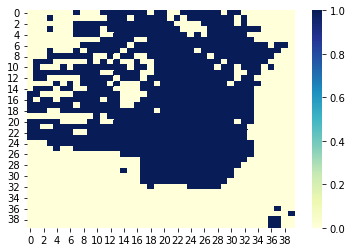
\includegraphics[width=1\linewidth, height=0.3\textheight]{pred_theft_hotspots.png}
        \caption{pred. hotspots}
    \end{subfigure}%
    \begin{subfigure}{0.32\textwidth}
        \centering
        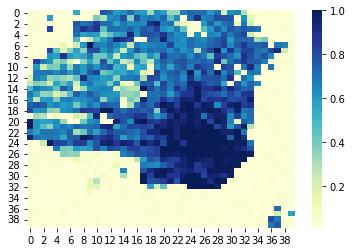
\includegraphics[width=1\linewidth, height=0.3\textheight]{pred_theft_prob.png}
        \caption{pred. prob.}
    \end{subfigure}
    }
\end{figure}
\end{frame}

\begin{frame}{Results}

\begin{figure}[!htb]
{\tiny
    \centering
    \begin{subfigure}{.5\textwidth}
        \centering
        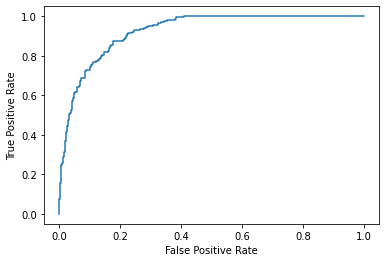
\includegraphics[width=0.7\linewidth]{ROC_robbery.png}
        \caption{Robbery ROC Curve \\
  (auroc = $0.925$)}
    \end{subfigure}%
    \begin{subfigure}{.5\textwidth}
        \centering
        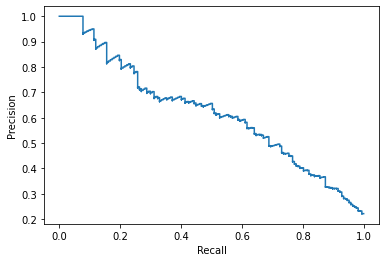
\includegraphics[width=0.7\linewidth]{PRC_robbery.png}
        \caption{Robbery Precision-Recall Curve \\
  (aps = $0.620$)}
    \end{subfigure}
    
    \begin{subfigure}{.32\textwidth}
        \centering
        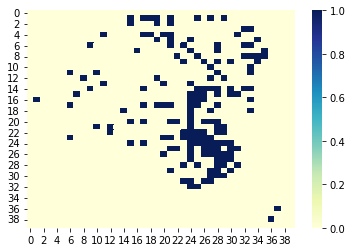
\includegraphics[width=1\linewidth, height=0.3\textheight]{true_robbery_hotspots.png}
        \caption{Robbery true hotspots}
    \end{subfigure}%
    \begin{subfigure}{0.32\textwidth}
        \centering
        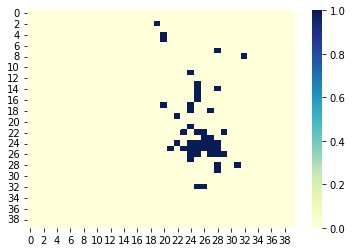
\includegraphics[width=1\linewidth, height=0.3\textheight]{pred_robbery_hotspots.png}
        \caption{pred. hotspots}
    \end{subfigure}%
    \begin{subfigure}{0.32\textwidth}
        \centering
        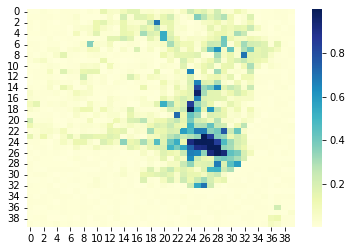
\includegraphics[width=1\linewidth, height=0.3\textheight]{pred_robbery_prob.png}
        \caption{pred. prob.}
    \end{subfigure}
    }
\end{figure}
\end{frame}






\begin{frame}{Conclusions}
\begin{itemize}
    \item Use VGGNet + LSTM to extract dynamic spatio-temporal features from incident maps
    \item Use AlexNet to extract static spatial features from satellite imagary
    \item Forecasting for ``All Crime'' performs better than specific crime type
    \item Explore more on the effect of satellite imagery
    \item Ethical issue with crime forecasting \citep{gstrein2019ethical}
\end{itemize}
\end{frame}






%----------------------------------------------------------------------------------------



%%



\begin{frame}[allowframebreaks]{References}
\bibliographystyle{abbrvnat}
\bibliography{bibfile.bib}
\end{frame}
%------------------------------------------------

\begin{frame}
\Huge{\centerline{Thank You}}
\end{frame}

%----------------------------------------------------------------------------------------

\end{document} 